\chapter{Implementation}
\lstset{language=NoBeardAsm}
\section{Used Technologies}
\subsection{IntelliJ IDEA} 
The Implementation of the project is written in Java on the integrated development environment IntelliJ which is mainly for developing Java based software. Nevertheless, it supports other programming languages too like Scala, Groovy and Kotlin. The IDE is also often used for mobile development in Android or Cordova. It could be very practicable for web development because of the different frameworks like JavaScript, AngularJs, Node.js, TypeScript etc…
This IDE support a huge variety of benefits such as:
\begin{itemize}
\item Different build systems (maven, gradle, ant, grunt, bower etc \ldots)
\item Version control systems (Git, Mercurial, Perforce, and SVN)
\item Plugin ecosystem
\item Test runner and coverage
\end{itemize}
\subsection{Maven} \label{sec:maven}
This is a software management and build automation tool which is based on the concept of a project object modem (POM). One of the biggest feature in Maven is the dependency management. Maven automatically downloads in POM file declared libraries and plug-ins from a repository and stores them local. The local repository is a folder structure that is used as a centralized storage place for locally built artifacts and as a cache for downloaded dependencies. The Maven command mvn install builds a project and places its binaries in the local repository. Then other projects can utilize this project by specifying its coordinates in their POMs.
\subsection{Scene Builder} \label{sec:SceneBuilder}
JavaFX Scene Builder is a visual layout tool that generates FXML, an XML-based markup language that lets developers to quickly design user interfaces, without any coding. Users just have to drag and drop UI components to the work area. By selecting components users can easily modify their properties or apply style sheets. The code for the layout is generated automatically in the background by the tool. The resulting FXML file can be combined with a Java project by binding the UI to the application’s logic. Every item of the layout view can be assigned with an fx:id to give the controller an easy access of components by the "@FXML" annotation.  SceneBuilder is an external tool so it has to be downloaded from the official Oracle website and has to be integrated to a Java supportive IDE. 
\subsection{JavaFX}
JavaFX enables developers to design rich client applications that is able to run constantly on different platforms. It offers a wide range of APIs for web rendering, user interface styling and media streaming. The newest JavaFX releases are fully integrated with the Java SE 7 Runtime Environment, which is available for all main desktop platforms. and the Java development Kit. So JavaFX application compiled to JDK 7 or later also run on all major desktop. 
\section{Surrounding packages}
The NoBeard Machine is part of the existing NoBeard project. This project already consists of the following packages:
\begin{itemize}
\item \textbf{asm: }NoBeard Assembler to assemble .na files 
\item \textbf{compiler: }NoBeard Compiler to compile .nb source code files
\item \textbf{config: }Hold information of the NoBeard project
\item \textbf{error: }To handle errors that are acquiring during compilation or assembly   
\item \textbf{io: }Responsible for reading source files and handling binary files 
\item \textbf{machine: }Implements a virtual machine with components like DataMemory, ProgramMemory, Instructions etc...  
\item \textbf{parser: }Converts source code files to binary files
\item \textbf{scanner: }To analyze NoBeard source code files for keywords, operands or arguments  
\item \textbf{symbolTable: }Looks up for matching words based on the symbol table entry  
\end{itemize}
However, one of the most important package is the “machine”. This is defined as the core of the whole project because it has the most significantly roles such as running a NoBeard program.
\section{Architecture of the User Interface}
The GUI is designed very similar to the Model-View-Controller pattern. However, this project is not depending on any database so it comes without any Model. The GUI project is build up of three main components as shown in figure~\ref{fig:partsOfGui}. The Controller and the Virtual Machine both of them is running on different threads and are accordingly synchronized. This will be described in detail in section~\ref{sec:synchronization}. The relationship between the controller and view is for event actions and updating of view-components like data memory, output or program flow. The View allows users to call functions from the Controller by clicking on control buttons or by entering inputs. 
\begin{figure}[h] 
	\centering
	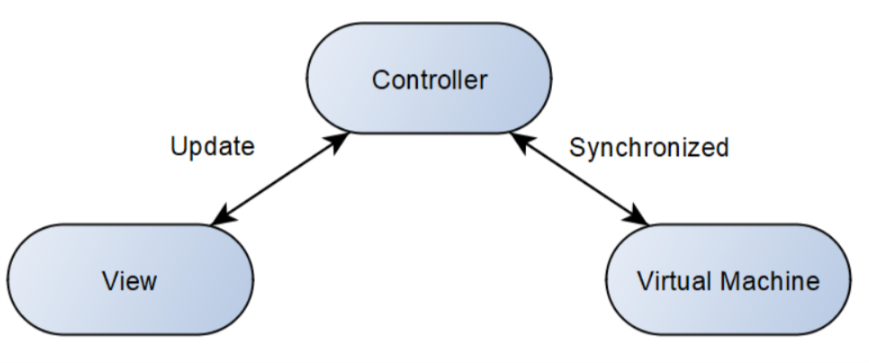
\includegraphics[scale=.70]{images/modelOfGui.png}
	\caption{Main parts of the GUI implementation}
	\label{fig:partsOfGui}
\end{figure}
\subsection{The View}
The view is basically a single \lstinline$.fxml$ file which holds the view components of the layout. As figure~\ref{fig:view} shows it was created with an external tool called Scene Builder which is already described in section~\ref{sec:SceneBuilder}. Each window is made up of an AnchorPane and is separated by SplitPanes. AnchorPane enables developers to construct high rated dynamic user interfaces for desktops. It is a highly specialized layout that can be used for edge alignment. This benefit gives the possibility to fill the whole pane to the parent, which is a SplitPane, by setting anchor offsets to zero. So, it becomes very comfortable and easy to size every window as the user wants. Then each of these AnchorPanes holds the needed view-components like Button, TextArea, TextField, ListView or ScrollPane. 
There are two types of designing and both of them is used in this project to develop an UI that meats all usability requirements.
\subsubsection{Static Design}
Static designing means that all view components are defined in the layout file and not in the Java code. With this type of designing it is pretty easy to build quickly a basic user interface. The developer has only to define the components in a fxml file or place them onto the view via drag and drop with the help of Scene Builder. This part of a project is mostly done by a designer because it does not require a lot of programming knowledge, just creativity. The code snippet~\ref{listing:XmlCode} shows a simplified version of how the control buttons were defined in the fxml file.
\lstset{language=XML,style=MyStyle}
\begin{lstlisting}[caption={FXML example}, label=listing:XmlCode]
<AnchorPane>
	<Button fx:id="openButton" onAction="#openFile" text="Open File"/>
	<Button fx:id="startButton" onAction="#startProgram" text="Run"/>
	<Button fx:id="stepButton" onAction="#step" text="Step"/>
	<Button fx:id="continueButton" onAction="#continueToBreakpoint" text="Continue"/>
	<Button fx:id="stopButton" onAction="#stopProgram" text="Stop"/>
</AnchorPane>
\end{lstlisting}

\subsubsection{Dynamic Design}
In dynamic design the already existing view is being changed according to run time or to user interactions. This means that the view changes only when a user or system triggers an event that matches a particular condition. In this case, the design code has to be mixed with the Java code and therefore programming skills from both sides are necessary. The code snippet~\ref{listing:ProgramDataView} shows a function which is called after a user opens a binary file. This function fills the program window with the content and additionally inserts to each line a CheckBox for the maintaining of breakpoints.

\lstset{
  language=Java,
  identifierstyle=\color{black},
  keywordstyle=\color{blue},       % keyword style
  stringstyle=\color{forestgreen},     % string literal style
}
  
\begin{lstlisting}[caption={Implementation of program data view},label=listing:ProgramDataView]
private void fillProgramDataView(List<String> programDataList) {
    VBox programData = new VBox();
    for (String lineStr : programDataList) {
        CheckBox line = new CheckBox(lineStr);
        line.setPadding(new Insets(1));
        line.setOnAction((event) -> {
            if (event.getSource() instanceof CheckBox) {
                CheckBox breakpoint = (CheckBox) event.getSource();
                if (breakpoint.isSelected())
                    machine.addBreakpoint(getAddressOfProgramLine(breakpoint.getText()));
                else
                    machine.removeBreakpoint(getAddressOfProgramLine(breakpoint.getText()));
            }
        });
        programData.getChildren().add(line);
        programDataMap.put(getAddressOfProgramLine(line.getText()), line);
    }
    programDataView.setContent(programData);
}
\end{lstlisting}

\begin{figure}[h] 
	\centering
	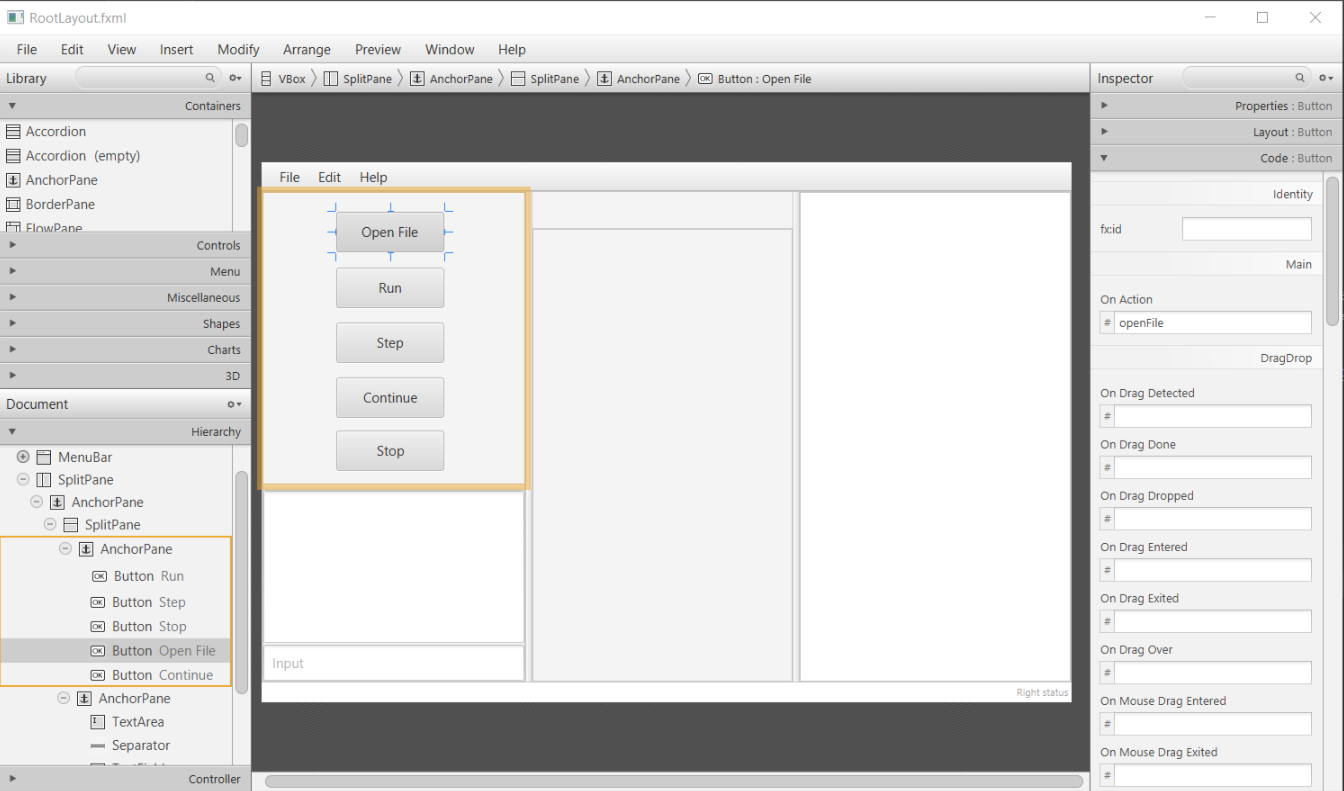
\includegraphics[scale=.55]{images/view.png}
	\caption{Development of the view with Scene Builder}
	\label{fig:view}
\end{figure}
\subsection{The Controller}
The controller is primarily responsible for the coordination and operation of the view and its components. As already described in section~\ref{sec:SceneBuilder} the controller can have easy access to the view components via the binding of an fx id. But firstly, they have to be connected with each other by setting the \lstinline$fx:controller$ attribute of the root view element to the currently used controller. Through this advantage it does not need to now the resource file of the layout or to call any "get" functions to get the target items. Even event actions, like mouse click or key pressing, can be bound between the controller and the view. This could be achieved by setting a name for the "On Action" property in Scene Builder and then creating the related function in the controller. The function has to be declared with the \lstinline$@FXML$ annotation and the same name as it was set on the action property of the item. Even functions like this comes only with a single argument which an ActionEvent. This parameter could be very helpful for getting some further information of the fired event like which mouse button was pressed.
The other big task that the controller has to handle is to execute user commands on the virtual machine. So it acts like a bridge to the machine and calls functions like run program, step one instruction further or view data etc\ldots 

Initially, the controller gets an instance of the NoBeard machine which is being target for NoBeard assembler programs. The opening of a NoBeard object file is operated with the help of a BinaryFileHandler. After a successful opening of the object file, it has to be disassembled. This means the disassembler has to convert the content of a binary file to primary program data where addresses, instructions and operands become visible on the GUI.
By finishing the translation, the machine has to load the strings and the program data from the object file into the corresponding memory. Program data is filled in a VBox where each line consists of a CheckBox and an Assembler statement. All of the CheckBoxes gets an OnAction event which adds and removes breakpoints from the machine. 
By starting to run a program, a new external thread has to be started where the machine runs separate from the UI. The code~\ref{listing:startingThread} illustrates how the machine gets started on a background thread using lambda expression.
\begin{lstlisting}[caption={Starting the machine on a new thread},label=listing:startingThread]
@FXML
void startProgram(ActionEvent event) {
    prepareGuiForProgramStart();
    new Thread(() -> {
        machine.runProgram(0);
        highlightNextInstructionToBeExecuted();
        Platform.runLater(() -> DataMemoryView.update(this, getRawDataMemoryList()));
    }).start();
}
\end{lstlisting}
The reason why and how they run on different threads will be explained in section~\ref{sec:synchronization}. The machine executes step by step every instruction of the program until any interruptions. It can be interrupted by a breakpoint, input request or by a \lstinline$halt$ instruction. 
\section{Synchronization of NoBeard Machine and GUI}
\label{sec:synchronization} 
As already mentioned the NoBeard virtual machine has to run on a background thread. The main reason for this is that there are two different processes using common processing resources. For instance, if they run on the same thread then the user would not be able to make any interactions because the virtual machine locks the main thread. But, even when the virtual machine gets an extra thread there would be still a deadlock because the background thread has to synchronize with the UI thread. So e.g., every time the user has to operate an input, a switch to the UI thread is needed. Otherwise it would cause a critical section between the threads. The synchronization of these two threads is implemented with the semaphore construction. A semaphore has a pretty simple usage to solve critical section problems and to achieve process synchronization in the multi processing environment. It is a variable that acts like a traffic light with its \lstinline$acquire()$ and \lstinline$release()$ functions.

The NoBeardMachine contains two interfaces to optimize outputs and inputs on the used device. As soon as the machine executes an input instruction \lstinline$in$, it calls firstly a function from the input interface either \lstinline$hasNextInt()$ or \lstinline$hasNext()$. Both do the same thing, checks whether there is an input by the user or not. The only different is that the one of them also checks if the string is numeric. These functions are overridden in the FxInputDevice class where also an instance of the controller is loaded by the constructor. So, by calling one of these hasNext function the machine thread should be paused as shown in the code snippet~\ref{listing:Synchronisation1}. To avoid the deadlock, the semaphore from the controller is acquired at this position i.e. at line~11.
\begin{lstlisting}[caption={Synchronisation with semaphore (Part 1)},label=listing:Synchronisation1]
@Override
public boolean hasNextInt() {
    waitForInput();
    return controller.getInput().chars().allMatch( Character::isDigit );
}

private void waitForInput() {
    try {
        controller.enableInputView(true);
        controller.getSemaphore().acquire();
    } catch (InterruptedException e) {
        e.printStackTrace();
    }
}
\end{lstlisting}
Now the user can make an input on the UI thread and submit it. To get back to the machine thread, the semaphore hast to be released after the user fires the submit event by pressing the ENTER key. This is demonstrated with the code fragment~\ref{listing:Synchronisation2} more precisely at line~12. Then the machine continues at the same position where the semaphore was acquired, at one of the has Next function and can analyse the provided input string.
\begin{lstlisting}[caption={Synchronisation with semaphore (Part 2)},label=listing:Synchronisation2]
inputView.setOnKeyPressed(event -> {
    if (event.getCode() == KeyCode.ENTER && inputView != null && 
    !inputView.getText().isEmpty())
        inputIsAvailable(inputView.getText());
});

private void inputIsAvailable(String providedInput) {
    getOutputView().appendText(providedInput + "\n");
    input = providedInput;
    inputView.clear();
    enableInputView(false);
    getSemaphore().release();
}
\end{lstlisting}
\section{Handling of Breakpoints}
Machine internal handling of breakpoints is done as described in \cite{bendersky_how_nodate}. The implementation for the maintaining of breakpoints is coded with a simple observer pattern design to keep ;the best performance of the virtual machine. The idea of this solution is pretty easy to understand. The machine runs only as long as it is in a \lstinline$running$ state. So, a new instruction is introduced, called \lstinline$break$ which sets the machine into a \lstinline$blocked$ state. This means at the same time that as soon as a user sets a breakpoint on a specified instruction, a change from the original to a \lstinline$break$ instruction is necessary.
The ControlUnit which is responsible for execution cycles in the virtual machine is going to be an observable class. Then a new Observer class is implemented which is called debugger that is holding all breakpoints in a HashMap.

\lstinline$private HashMap<Integer, Byte> breakpoints;$
 
This HashMap stores the address and the instruction of a selected breakpoint. The debugger class contains in all three major functions as shown in the code snippet~\ref{listing:debugger}. Adding, removing breakpoints to or from the HashMap and replacing an instruction at a specified address from the program memory to a new one. The selection of a breakpoint on the UI calls the set or remove function from the debugger, as the case may be. As soon as a breakpoint is selected, it will be stored to the HashMap with its original instruction and at same time replaces the original instruction by the newly added \lstinline$break$ instruction.
\begin{lstlisting}[caption={Implementation of the debugger},label=listing:debugger]
void setBreakpoint(Integer address, Byte instructionId) {
    this.breakpoints.put(address, instructionId);
    programMemory.replaceInstruction(address, InstructionSet.Instruction.BREAK.getId());
}

void removeBreakpoint(Integer address) {
    programMemory.replaceInstruction(address, breakpoints.get(address));
    this.breakpoints.remove(address);
}

public void replaceInstructionAtAddress(int address, InstructionSet.Instruction instruction) {
    if (!breakpoints.isEmpty() && breakpoints.keySet().contains(address)) {
        if (instruction != null)
            programMemory.replaceInstruction(address, instruction.getId());
        else
            programMemory.replaceInstruction(address, breakpoints.get(address));
    }
}
\end{lstlisting}
This break instruction sets the machine to a \lstinline$blocked$ state and notify the observer to change the break instruction back to the original one which is stored in the HashMap. Now the machine is blocked at a specified breakpoint and the user can take a look to the current stack frames and go one step further in the program or continue the execution cycle to a next breakpoint. However, when the user wants to step further to execute the current instruction where the breakpoint is, of course again a switch back to the break instruction is needed after the original instruction completed.  
\section{Visualisation of DataMemory}
\label{sec:implementationOfDataVisualisation}
The visualisation of the data memory gives an overview about string constants and stack frames. As figure~\ref{fig:dataMemoryView} shows the view lists four byte of data on each row starting with the belonging address. Logically, the list has to be updated after any interruption by a breakpoint. This is demonstrated with the code snippet~\ref{listing:startingThread}, more precisely at line~7.
For the visualisation of these data a ListView is defined on the view which is one of the best choice for this purpose. 
\begin{figure}[h] 
	\centering
	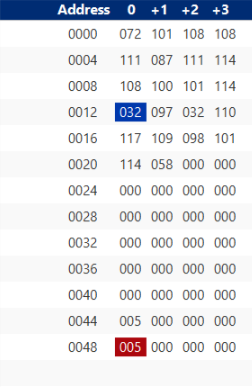
\includegraphics[scale=.99]{images/dataMemory.png}
	\caption{Visualisation of data memory}
	\label{fig:dataMemoryView}
\end{figure}
The updating of data memory view has defined a cycle. Firstly a function iterates through the memory until the current stack pointer and groups all data into four bytes and finally stores them into an observable collection of strings. Then this collection is assigned to ListView items that are visible on the view. Each row of the ListView contains now a line of string filled with the address and four pure data. Since each item in a ListView is represented by an instance of the ListCell class, a row can be customized to get a nice structure like in figure~\ref{fig:dataMemoryView}. This customisation of a cell can be achieved with the cellFactory API. The cell factory is called by the platform whenever it determines that a new cell needs to be created. 
To specialize the Cell used for the ListView, an implementation of the cellFactory callback function has to be provided.
\begin{lstlisting}[caption={Implementation of the data memory view using cell factory},label=listing:CellFactory]
static void update(Controller controller, ObservableList<String> content) {
    controller.getDataMemoryListView().setItems(content);
    controller.getDataMemoryListView().setCellFactory(list -> new ListCell<String>() {
        int framePointer = controller.getMachine().getCallStack().getFramePointer();
        int stackPointer = controller.getMachine().getCallStack().getStackPointer();
        static final int INDEX_OF_ADDRESS = 0;

        @Override
        protected void updateItem(String item, boolean empty) {
            super.updateItem(item, empty);
            if (item != null) {
                createDataLine(item);
            }
        }

        private void createDataLine(String item) {
            HBox line = new HBox();
            int firstAddressInLine = getIndex() * 4;
            convertStringToLabels(firstAddressInLine, item).forEach(line.getChildren()::add);
            setContextMenuToDataCells(line);
            setGraphic(line);
        }

        private List<Label> convertStringToLabels(int firstAddressInLine, String line) {
            String[] lineContent = splitDataLine(line);
            List<Label> result = createLabelForAddress(lineContent[INDEX_OF_ADDRESS]);
            int currentAddress = firstAddressInLine;
            for (int i = 1; i < lineContent.length; i++) {
                if (currentAddress == framePointer)
                    result.add(createHighlightedLabel(lineContent[i], "#0038AC"));
                else if (currentAddress == stackPointer)
                    result.add(createHighlightedLabel(lineContent[i], "#AC080E"));
                else
                    result.add(createNormalLabel(lineContent[i]));
                currentAddress++;
            }
            return result;
        }
        ...
\end{lstlisting}
In the code example~\ref{listing:CellFactory} an anonymous inner class is created using modern lambda expression, that simply returns instances of ListCell overriding the updateItem method. This method is called whenever the item in the cell changes, for example when the user scrolls the ListView or the NoBeard machine updates the data memory (and the cell is reused to represent some different item in the ListView). Because of this, there is no need to manage bindings - simply react to the change in items when this method occurs. In this example, whenever the item changes, we update the cell text property, and also modify the text fill to ensure that we get the correct visuals.
So each row of the list view will be separated in five labels, one for the address and four with one byte data. Labels with a given id can be easily styled in a extra CSS file by setting paddings or backgroundcolor. The data labels get a click event to open up a context menu where four functions are available:
\begin{itemize}
\item Convert data to a single character
\item Convert a line of data to four characters
\item Convert a line of data to a single integer
\item Convert a translated line of data back to raw data
\end{itemize}
For the implementation of these functions a separated \lstinline$DataMemoryConverter$ class is introduced. The conversion of a single byte to character is handled by translating the ASCII value which is the current byte to a char. For integers it is a bit more complex because a single integer has to take four byte of data. So if all the four bytes are not aligned in one row, the rest bytes has to be occupied from the next row. And integers are stored in little endian order, that means the lowest significant byte is stored first. 